\chapter{Non-parametric Regression}

\section{}

The two kernel functions chosen are the \textbf{Gaussian} kernel and the \textbf{Epanechnikov} kernel. We have used \textbf{k-fold cross-validation} to find the bandwidth corresponding to minimum estimated risk for each kernel. For estimating risk, the data was shuffled using \texttt{pandas.DataFrame.sample} method. The data was then split into $k=10$ folds to perform cross-validation. The code can be found in \texttt{code/4.ipynb}. 

\section{}

The optimal bandwidths found are:

\begin{center}
  \begin{tabular}{| c | c |}
    \hline
    Kernel & Optimal bandwidth \\
    \hline
    Gaussian & 0.13183673469387755 \\
    Epanechnikov & 0.49734693877551023 \\
    \hline
  \end{tabular}
\end{center}
The plots obtained for the Gaussian kernel are:
\begin{figure}[H]
    \centering
    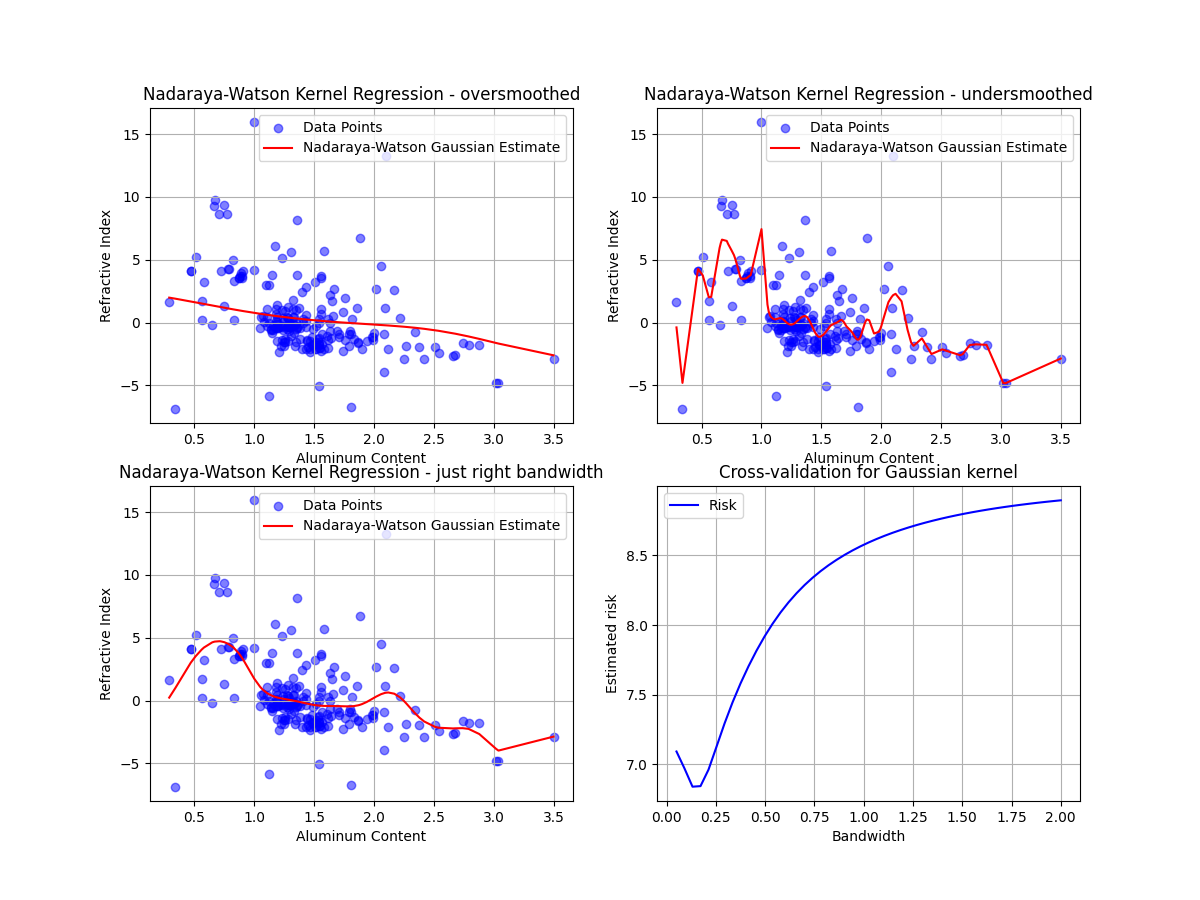
\includegraphics[width=0.6\linewidth]{assets//images/gaussian_kernel_regression.png}
    \caption{Gaussian kernel}
    \label{fig:4.1}
\end{figure}
The plot obtained for the Epanechnikov kernel are:
\begin{figure}[H]
    \centering
    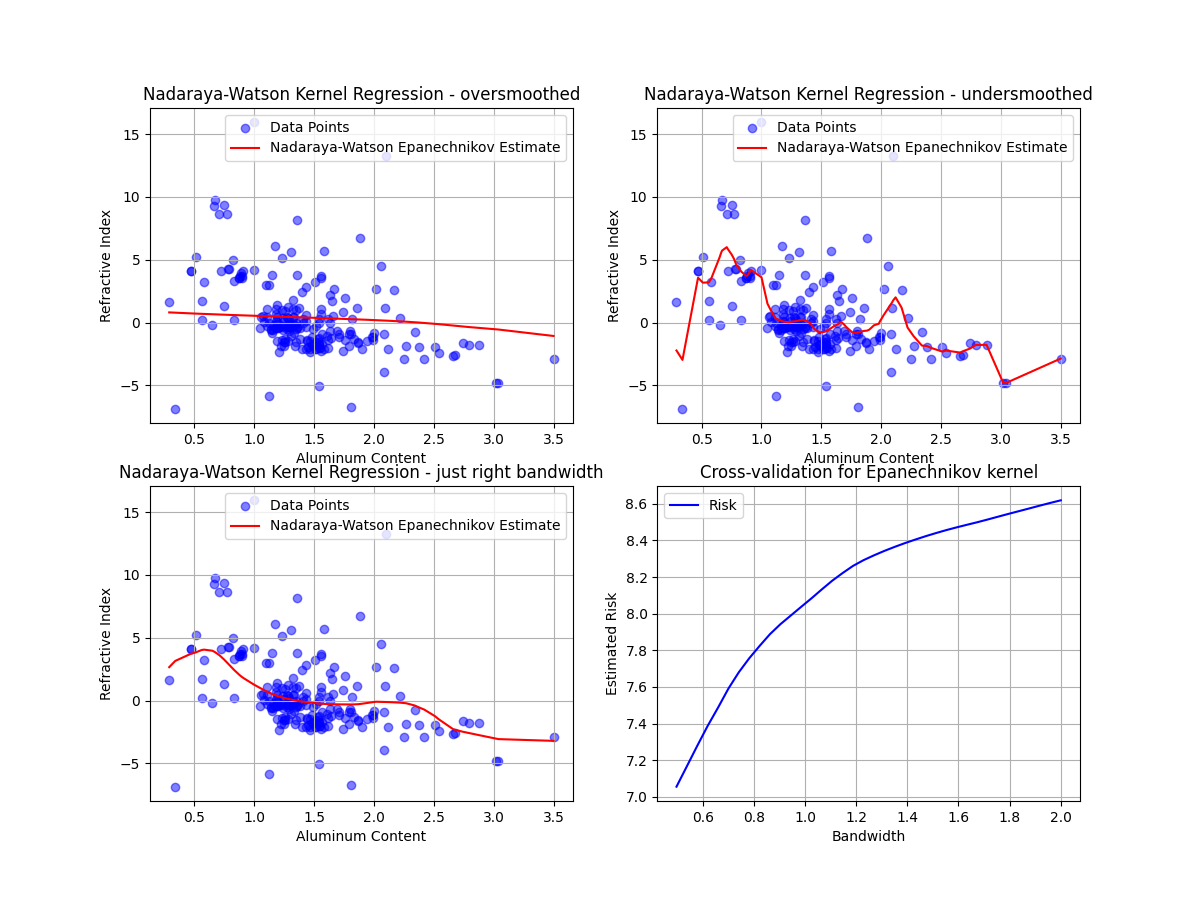
\includegraphics[width=0.6\linewidth]{assets//images/epanechnikov_kernel_regression.png}
    \caption{Epanechnikov kernel}
    \label{fig:4.2}
\end{figure}

\section{}

The Gaussian kernel gives a lower minimum risk than the Epanechnikov kernel. The values on on one run are:
\begin{center}
  \begin{tabular}{| c | c |}
    \hline
    Kernel & Minimum risk \\
    \hline
    Gaussian & 6.85 \\
    Epanechnikov & 7.21 \\
    \hline
  \end{tabular}
\end{center}

\subsection{Differences}
This shows that Gaussian kernel is better for this dataset. The risk-bandwidth graph for the Gaussian kernel reaches a minimum and then increases. On the other hand, the risk-bandwidth graph for the Epanechnikov kernel starts suddenly and then increases. For smaller bandwidth than the start point (the minimum-risk bandwidth), the risk tends to $\infty$ as the value $\left|\frac{x - x_i}{h}\right|$ is always greater than 1 for the given data.

\subsection{Similarities}
Some similarities between regression using both kernels are: the risk increases for large bandwidth. On overlapping the curves, both curves are found to be similar, as seen below
\begin{figure}[H]
    \centering
    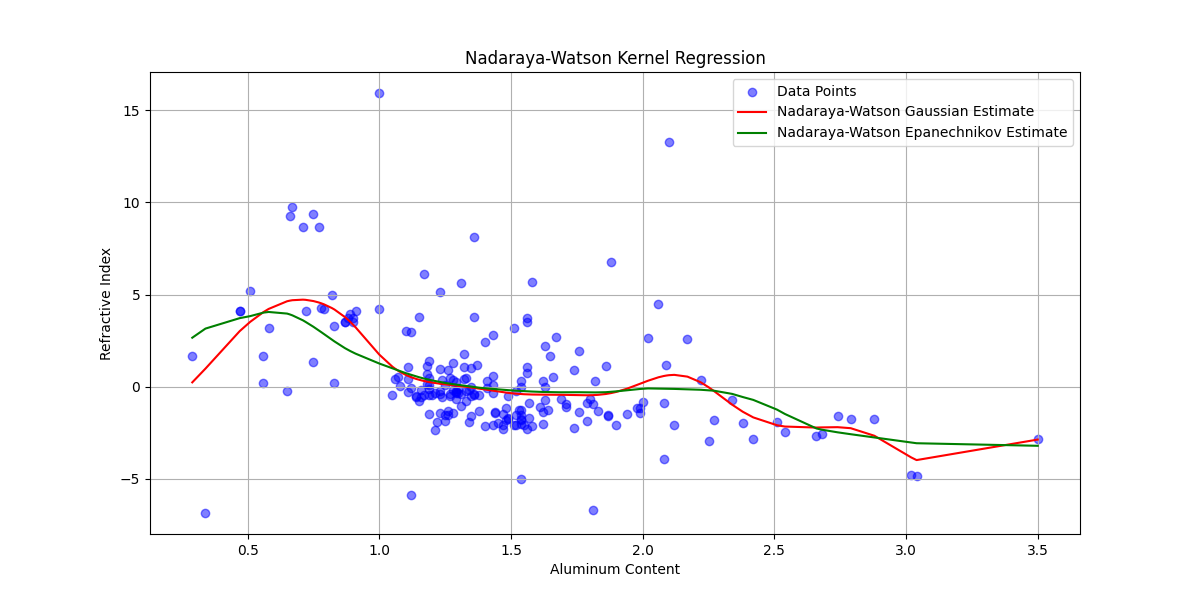
\includegraphics[width=0.6\linewidth]{assets/images/overlapped_kernel_regression.png}
    \caption{Overlapped plots}
    \label{fig:4.3}
\end{figure}

